\subsection{Figma Design}\label{figma_design}


\begin{minipage}{0.6\textwidth}
    Zur Erstellung eines Mockup des Designs für die \acs{gui} der \acs{rltanzeige} wurde Figma verwendet. Figma Design ist eine Applikation zum erstellen von Prototypen im Bereich \ac{uxui}. Dabei kann im Team in Echtzeit zusammen gearbeitet werden. Mit Figma können in das erstellte Design direkt interaktive Funktionen eingebaut werden, um ein realistisches Prototyping zu ermöglichen. Ein weiterer Vorteil von Figma ist der sog. \enquote{Dev Mode}. Mit diesem können Entwickler direkt auf das Design zugreifen und Details finden, die benötigt werden, um das Design in Code umzusetzen. \cite[vgl.][]{figma_design:o.J.}
\end{minipage}%
\hfill
\begin{minipage}{0.37\textwidth}
	\centering	
	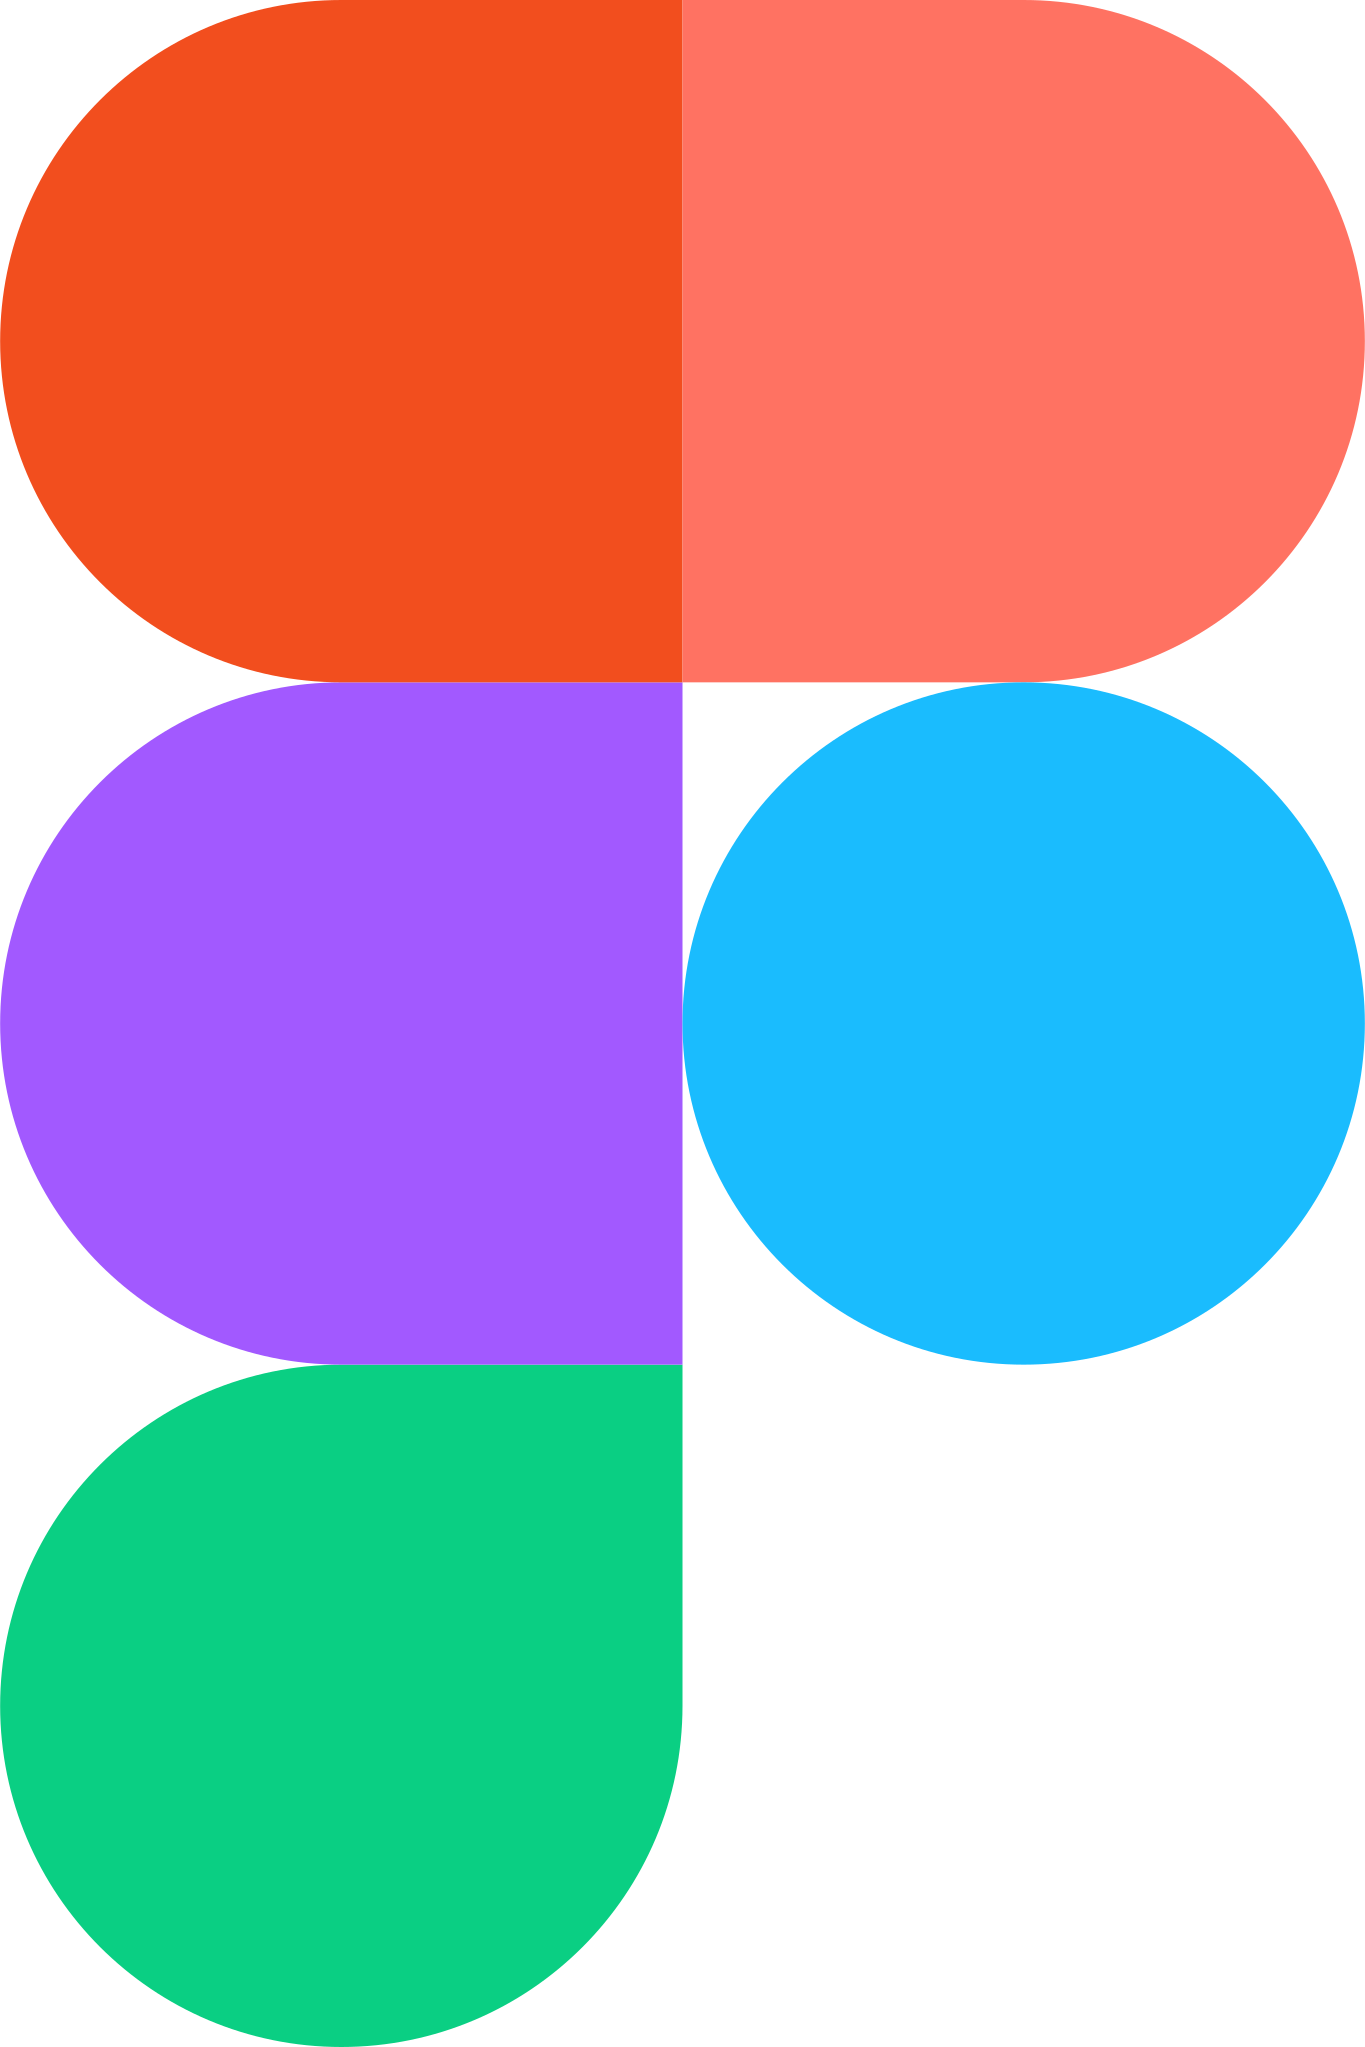
\includegraphics[width=0.50\textwidth]{figma_logo}
	\captionof{figure}{Figma Logo (Quelle: 
		\url{https://en.m.wikipedia.org/wiki/File:Figma-logo.svg}) \label{fig:figma_logo}}
\end{minipage}
\vspace{1ex}

Bei Erstellung des Designs lag die Priorität hauptsächlich auf Übersichtlichkeit. Die Vorgabe ...